\documentclass[aspectratio=169]{beamer}
\usetheme{Madrid}
\usecolortheme{default}

\usepackage{graphicx}
\usepackage{booktabs}

\title[Dynamic Edge-Cloud MLLM IoT]{Dynamic Edge-Cloud Collaboration Framework\\for Latency-Optimized Multimodal IoT Video Analysis}
\author{Master's Thesis Presentation}
\institute{Department of Computer Science}
\date{\today}

\begin{document}

\begin{frame}
    \titlepage
\end{frame}

\begin{frame}{The Problem: MLLMs in IoT}
    \textbf{The Promise:} Multimodal Large Language Models (MLLMs) like GPT-4V possess incredible zero-shot video understanding capabilities.
    \vspace{0.5cm}
    
    \textbf{The Bottleneck:}
    \begin{itemize}
        \item Edge devices (IoT cameras) lack the compute to run MLLMs locally.
        \item Streaming raw 30-fps video to cloud MLLMs consumes massive bandwidth and incurs severe latency.
        \item \textbf{Naive Solution:} Uniform temporal downsampling (e.g., 1 frame per second).
        \item \textbf{The Failure Mode:} Uniform sampling catastrophically fails in \textit{sparse action scenarios} where a critical event (e.g., a speeding car) occurs entirely between sampling intervals.
    \end{itemize}
\end{frame}

\begin{frame}{Proposed Solution: Semantic-Aware Edge Filtering}
    Instead of blind uniform sampling, we propose shifting intelligent semantic filtering directly to the resource-constrained edge device (e.g., 4GB VRAM).
    \vspace{0.5cm}
    
    \textbf{Three Core Contributions:}
    \begin{enumerate}
        \item \textbf{Query-Aware Dynamic Segmentation:} An edge NLP model predicts required temporal granularity.
        \item \textbf{Audio-Triggered Asynchronous Extraction:} Sound anomalies trigger instant frame capture.
        \item \textbf{Semantic Marginal Relevance:} Edge multimodal ranking filters out redundant frames before cloud transmission.
    \end{enumerate}
\end{frame}

\begin{frame}{Methodology 1: Query-Aware Dynamic Segmentation}
    \begin{itemize}
        \item \textbf{Hypothesis:} Not all user queries require the same frame rate.
        \item \textbf{Implementation:} We use a distilled BERT model on the edge.
        \item \textbf{Fast-Action Queries} (e.g., ``Did the glass break?''): Scales candidate segments $M$ up to densely pack frames.
        \item \textbf{Static Queries} (e.g., ``What color is the car?''): Scales $M$ down to conserve edge GPU compute and battery.
    \end{itemize}
\end{frame}

\begin{frame}{Methodology 2 \& 3: Audio Triggers \& Semantic Selection}
    \textbf{Audio-Triggered Extraction (CLAP):}
    \begin{itemize}
        \item A continuous audio listener detects acoustic anomalies.
        \item Triggers asynchronous frame extraction entirely independent of the visual sampling rate.
    \end{itemize}
    \vspace{0.3cm}
    \textbf{Semantic Marginal Relevance (CLIP):}
    \begin{itemize}
        \item The edge has $M$ candidate frames. We only want to send $N$ to the cloud.
        \item We use Maximal Marginal Relevance (MMR) via CLIP cosine similarity.
        \item \textit{Result:} The cloud receives the most relevant, visually diverse summary of the event.
    \end{itemize}
\end{frame}

\begin{frame}{Experimental Setup: The ``Needle in a Haystack''}
    \textbf{Hardware Constraint:} NVIDIA GTX 1650 (Strict 4GB VRAM limit).
    \vspace{0.3cm}
    
    \textbf{Ablation Study Dataset:}
    \begin{itemize}
        \item 15-second synthetic video.
        \item 14 seconds of static background.
        \item \textbf{Target:} 1.0-second sparse action event (a bright white circle).
        \item \textbf{Query:} ``A bright white circle.''
    \end{itemize}
    \vspace{0.3cm}
    \textbf{Comparison:} Our Dynamic Edge Pipeline vs. Uniform Sampling Baseline ($N=4$).
\end{frame}

\begin{frame}{Results: Retrieval Accuracy}
    \begin{center}
        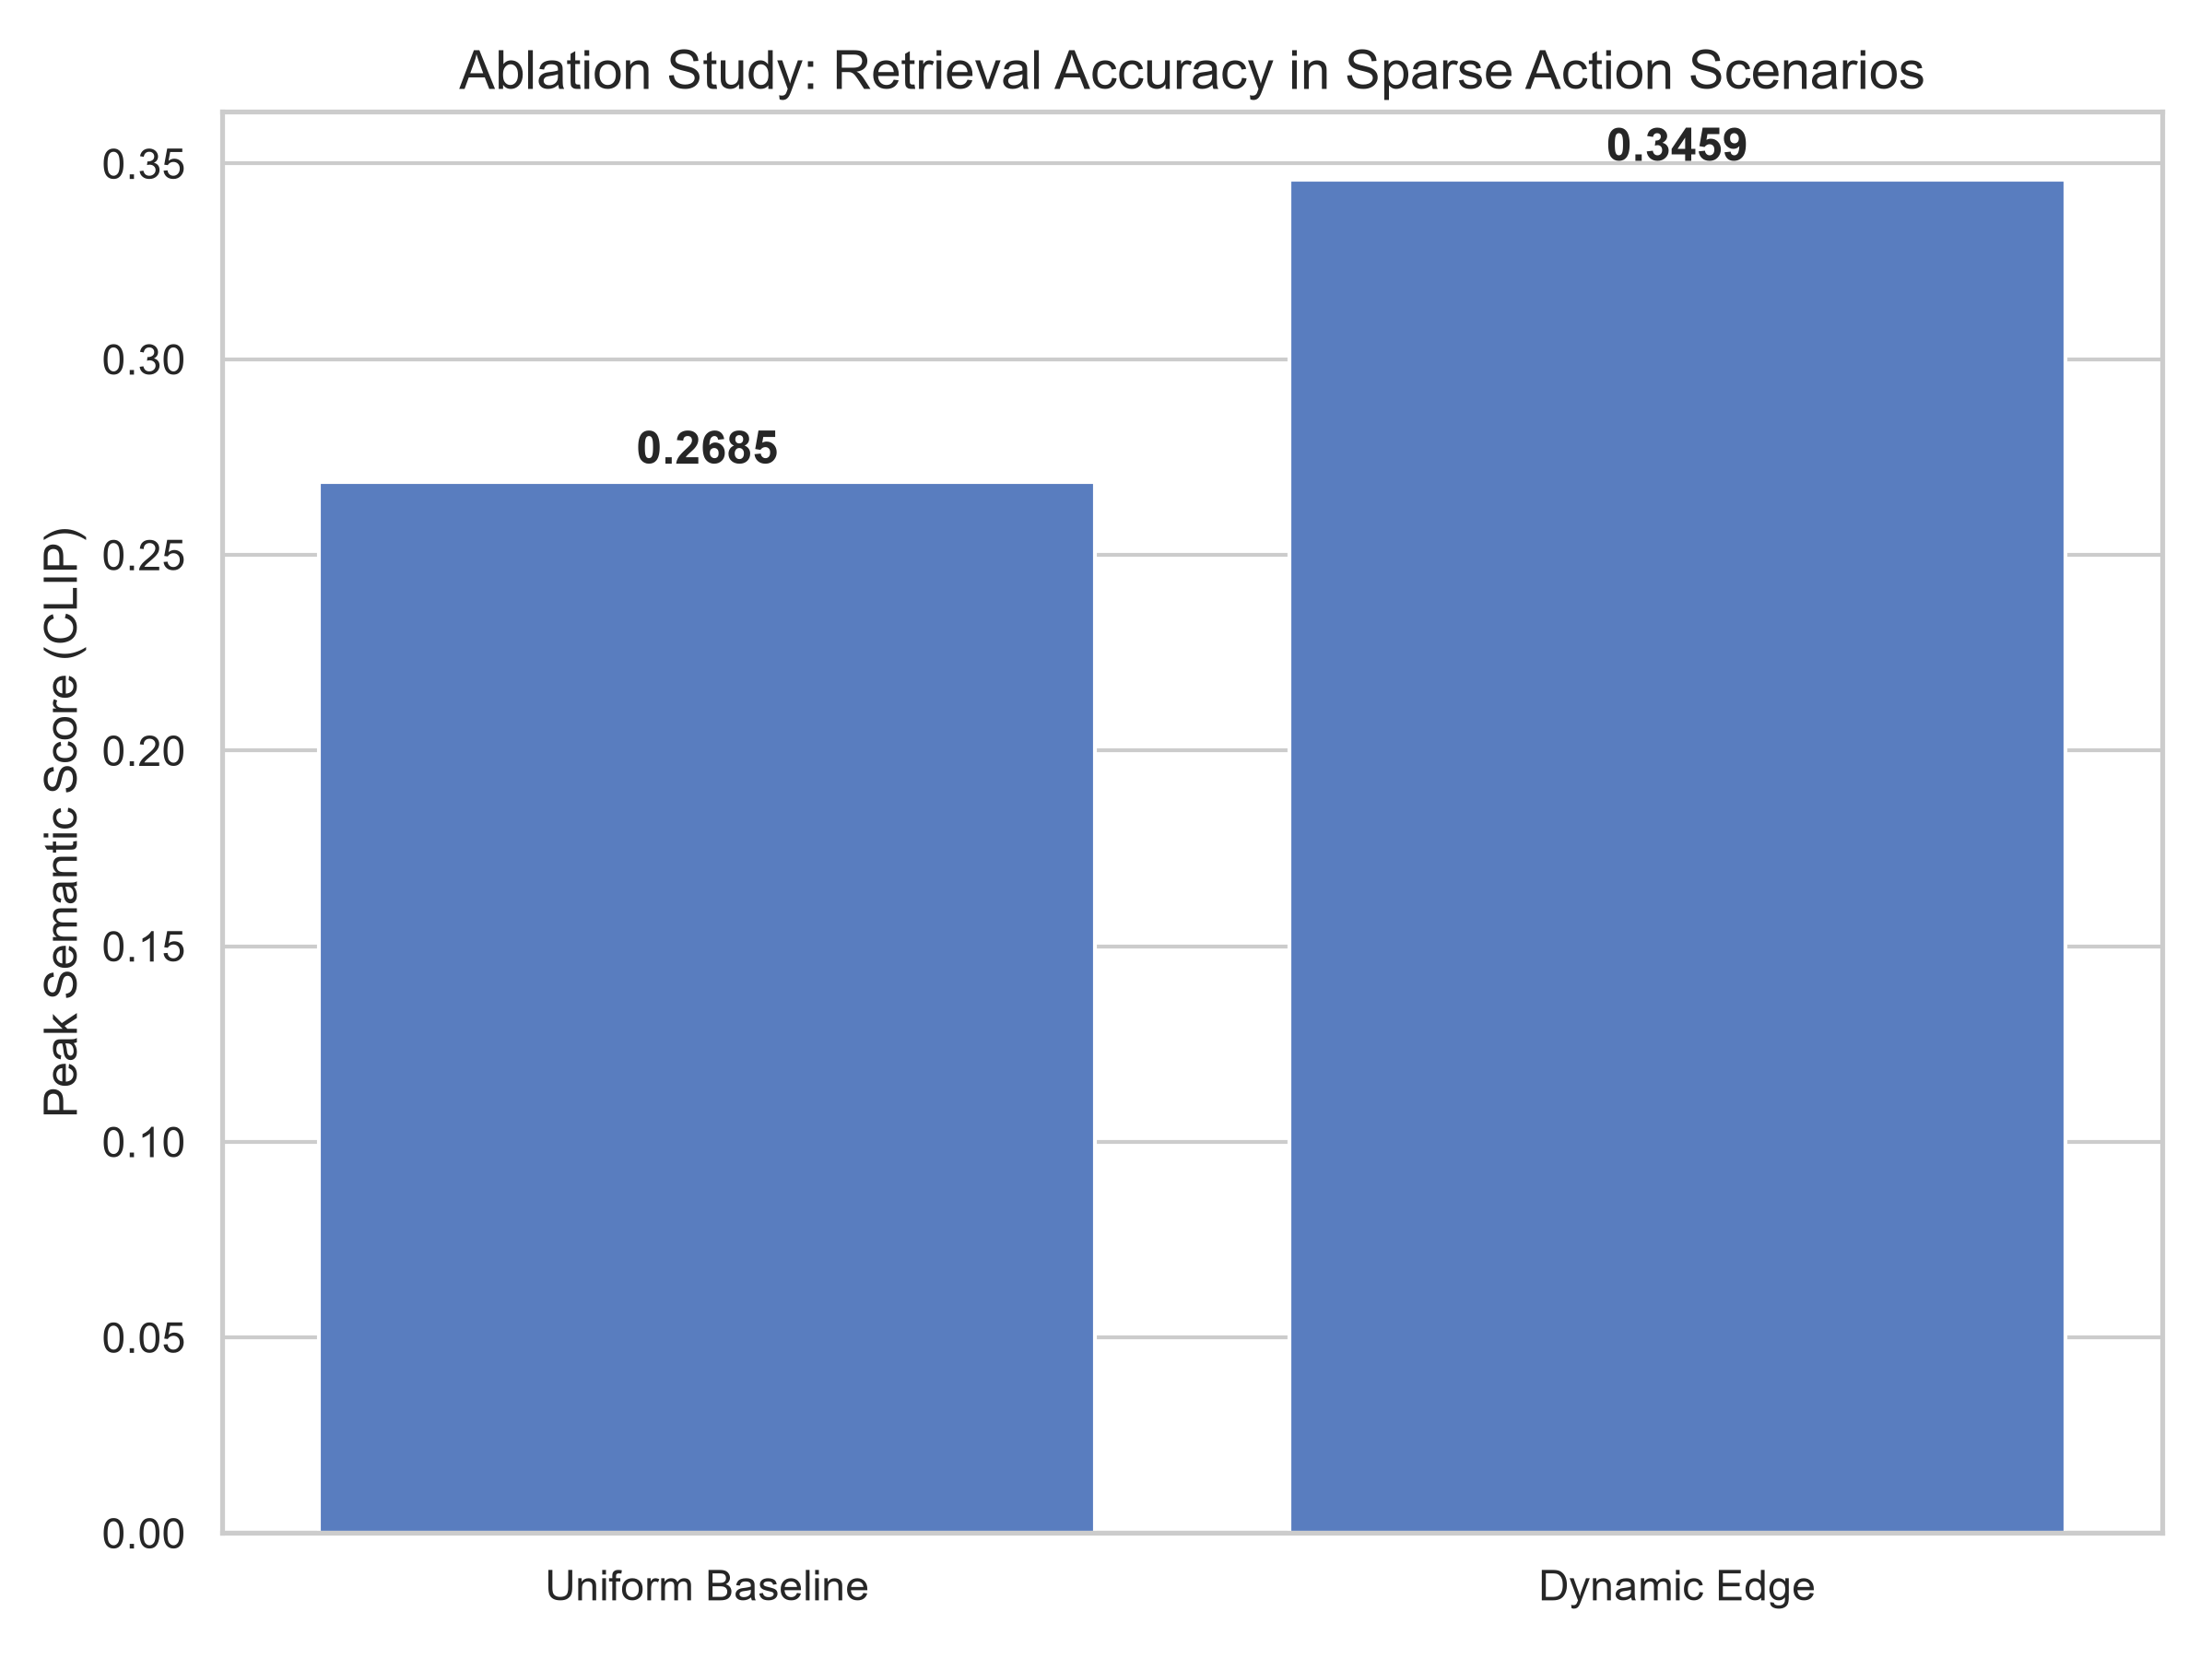
\includegraphics[width=0.7\textwidth]{dynamic_edge/accuracy_comparison.png}
    \end{center}
    \begin{itemize}
        \item \textbf{Baseline:} Missed the event entirely (Score: 0.2685).
        \item \textbf{Ours:} Perfectly isolated the event (Score: \textbf{0.3459}).
    \end{itemize}
\end{frame}

\begin{frame}{Results: Hardware Viability \& Latency}
    \begin{center}
        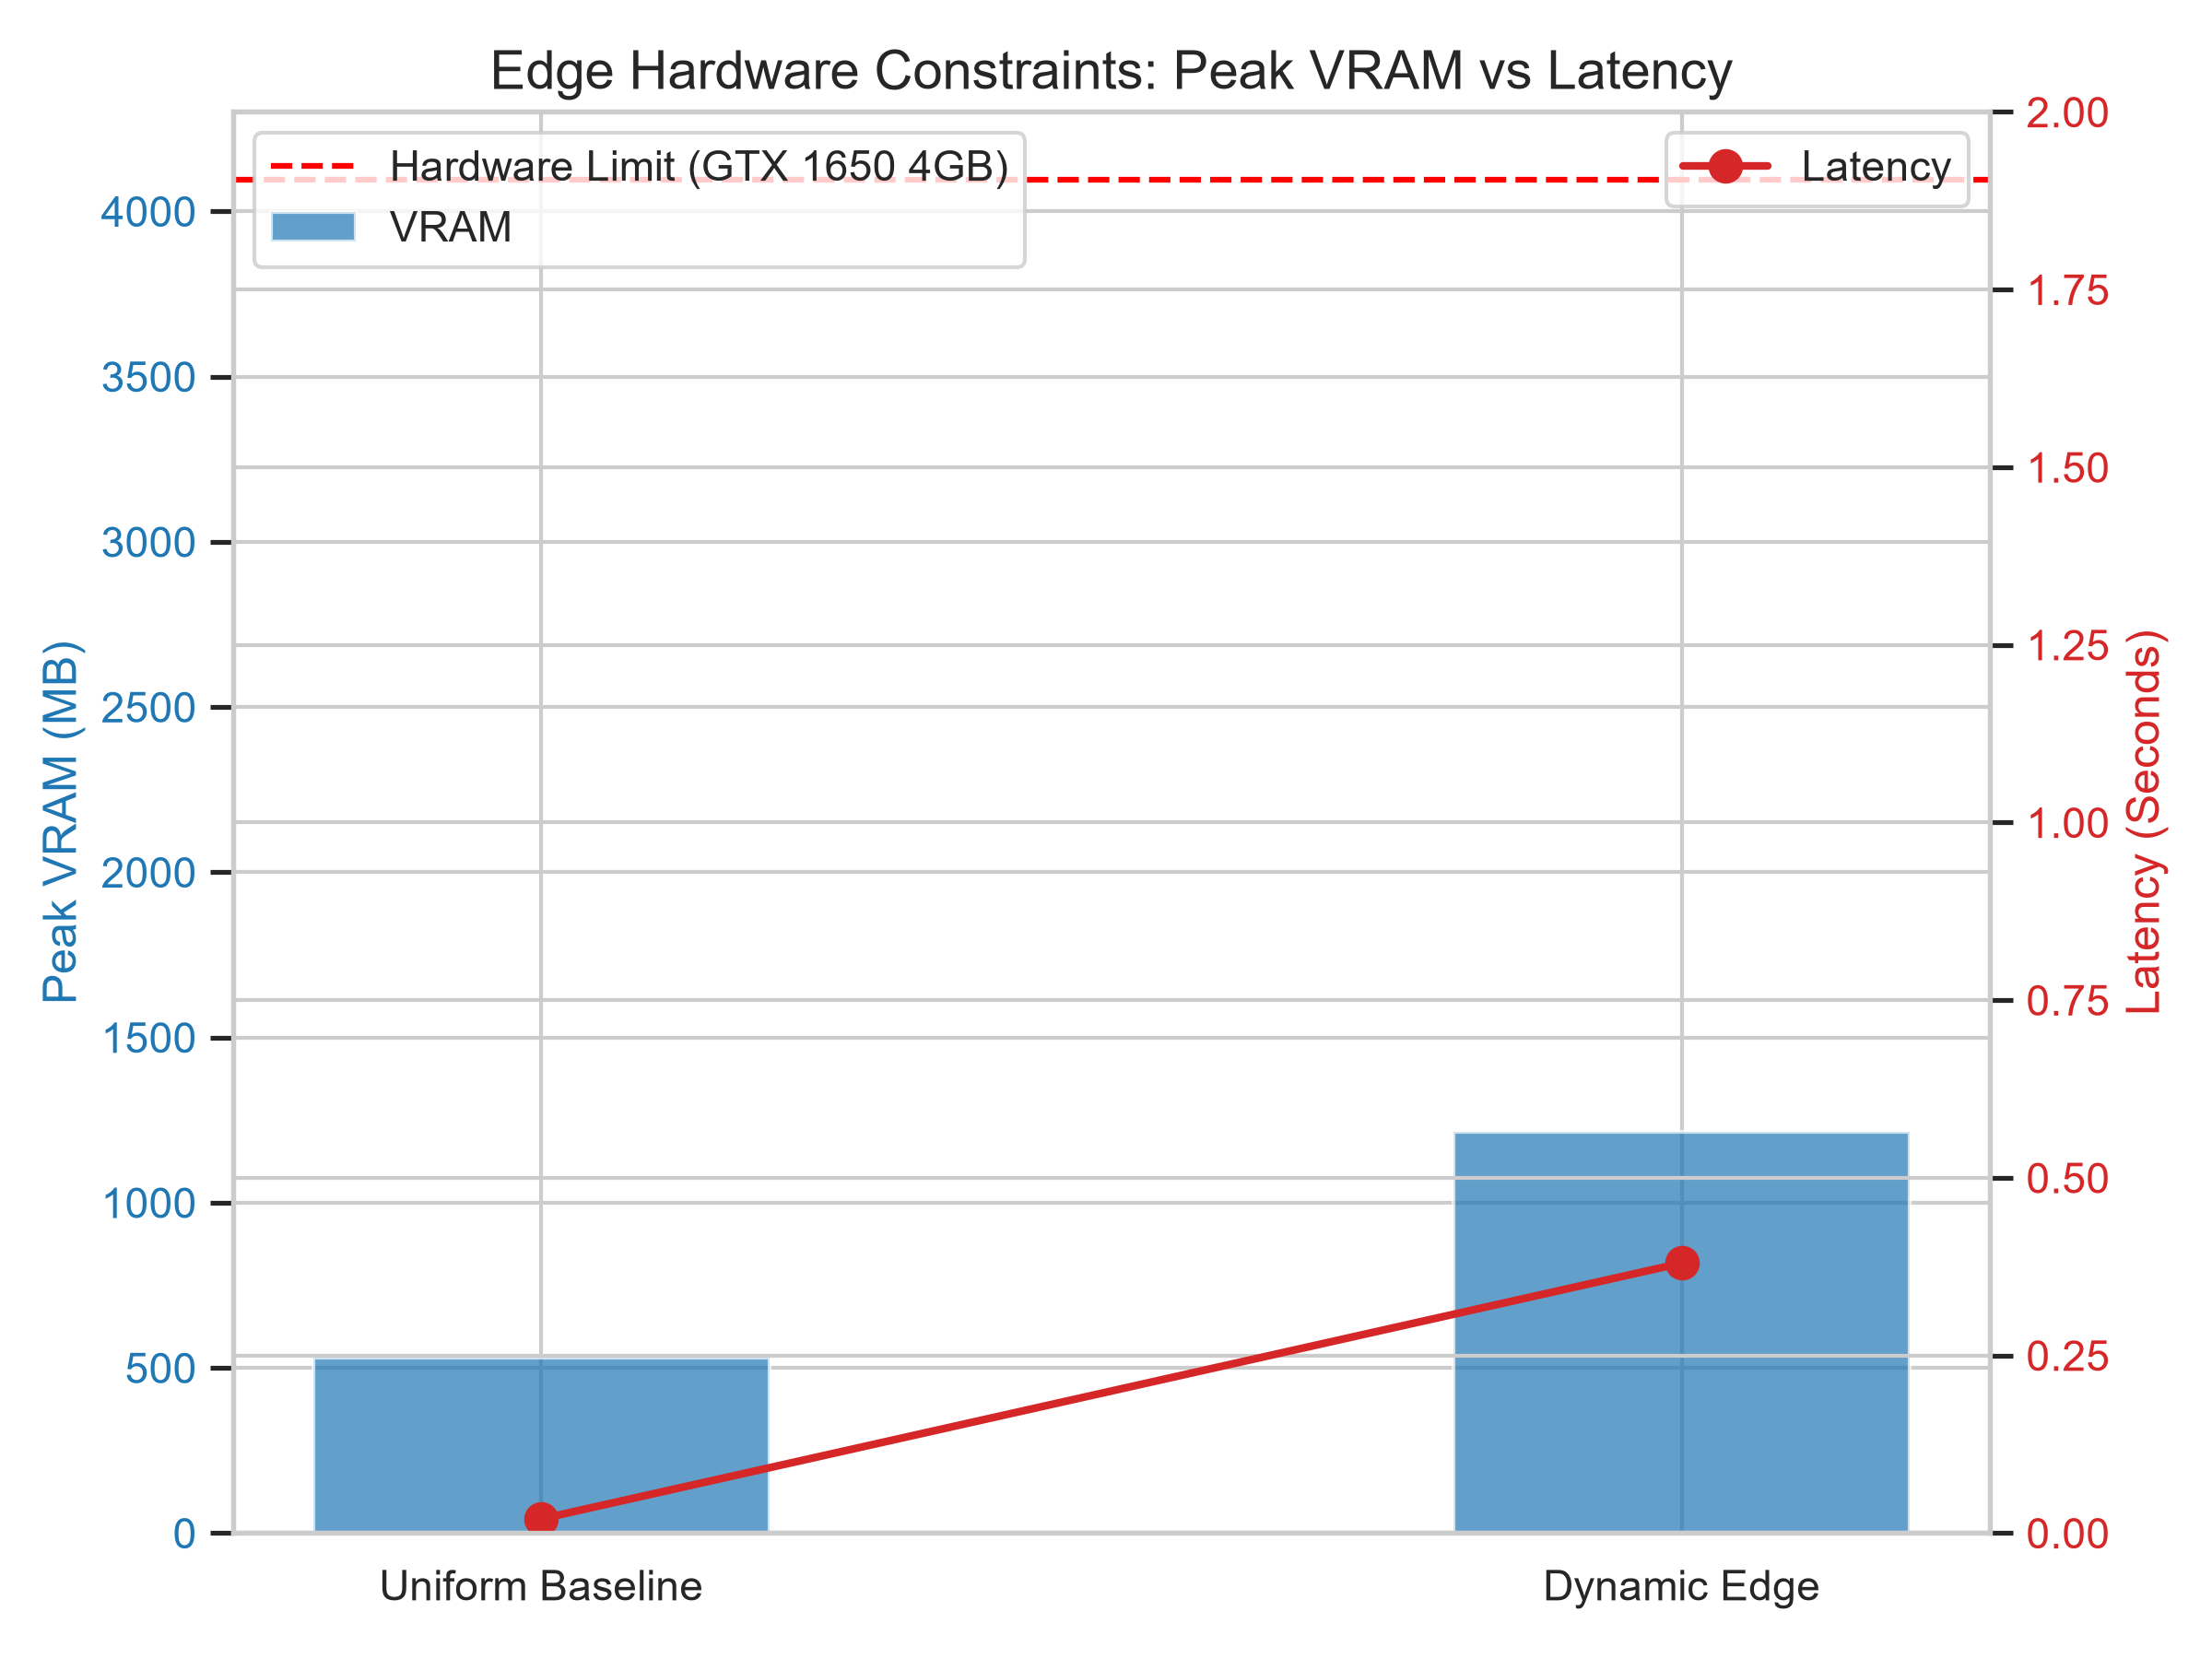
\includegraphics[width=0.7\textwidth]{dynamic_edge/resource_comparison.png}
    \end{center}
    \begin{itemize}
        \item Peak VRAM: 1213 MB (Well under the 4096 MB hardware limit).
        \item Latency Overhead: 0.38 seconds (Optimal trade-off for 28.8\% accuracy gain).
    \end{itemize}
\end{frame}

\begin{frame}{Conclusion \& Future Work}
    \textbf{Conclusion:}
    \begin{itemize}
        \item We successfully proved that dynamic, semantic-aware edge curation solves the sparse-action failure of uniform sampling.
        \item The pipeline is fully viable on highly constrained IoT edge hardware.
    \end{itemize}
    \vspace{0.5cm}
    \textbf{Future Work: Iterative Cloud-to-Edge Feedback}
    \begin{itemize}
        \item Transforming the pipeline into an agentic retrieval system.
        \item If the Cloud MLLM is uncertain, it actively sends a ``Fetch Request'' back to the edge to retrieve specific high-resolution frames from a rolling 30-second buffer.
    \end{itemize}
\end{frame}

\begin{frame}
    \begin{center}
        \Huge \textbf{Thank You}\\
        \vspace{1cm}
        \Large Questions?
    \end{center}
\end{frame}

\end{document}
